% AY2017 制御工学 解答例
% 回答の流れ・言葉遣いは 03_制御工学/参考/「制御工学Ⅱ（完成版）」に寄せる。
% デザイン（囲み枠等）は真似しない。解答・数値は本年度過去問から自力で導いた。
\documentclass[11pt,a4paper]{article}
\usepackage{../../../00_common/preamble}

\usetikzlibrary{positioning,arrows.meta,calc}
\usepackage{pgfplots}
\pgfplotsset{compat=newest}

\title{制御工学 AY2017 解答例（専門応用科目I）}
\author{}
\date{}

\begin{document}
\maketitle

% ==================================================================
\section*{第1問〔I〕}

二次振動系（質量 $m$、粘性係数 $d$、ばね定数 $k$）。

\subsection*{(1) 運動方程式と伝達関数}
\begin{align*}
  &\qquad m\ddot{x}+d\dot{x}+kx=f(t)\\
  &\therefore\quad (ms^2+ds+k)X(s)=F(s)
   \quad\therefore\quad G(s)=\frac{1}{ms^2+ds+k}.
\end{align*}
\[
  \therefore\quad \ans{\;m\ddot{x}+d\dot{x}+kx=f(t),\qquad G(s)=\dfrac{1}{ms^2+ds+k}\;}
\]

\subsection*{(2) $d,k$ と無減衰自由応答（$m=1,\omega_n=1,\zeta=0$）}
$\omega_n^2=\dfrac{k}{m}$、$2\zeta\omega_n=\dfrac{d}{m}$ より
\begin{align*}
  &\qquad k=m\omega_n^2=1,\qquad d=2\zeta\omega_n m=0.
\end{align*}
$f=0$ より $\ddot{x}+x=0$。$x=A\cos t+B\sin t$ に $x(0)=1,\dot x(0)=0$ を入れて $A=1,B=0$。
\[
  \therefore\quad \ans{\;d=0,\quad k=1,\quad x(t)=\cos t\;}
\]
減衰がないので振幅 $1$ の持続振動となる。

\begin{center}
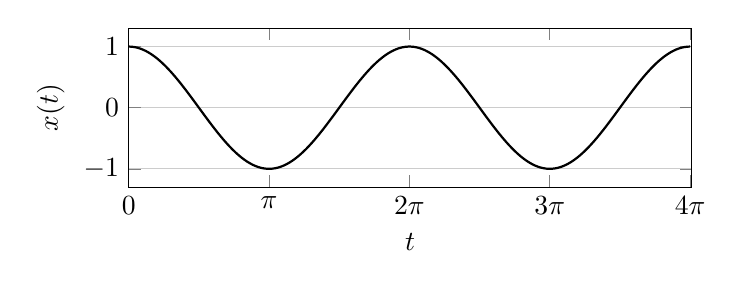
\begin{tikzpicture}
\begin{axis}[
  width=0.72\linewidth, height=3.6cm,
  xmin=0, xmax=12.6, ymin=-1.3, ymax=1.3,
  xlabel={$t$}, ylabel={$x(t)$},
  xtick={0,3.1416,6.2832,9.4248,12.566},
  xticklabels={$0$,$\pi$,$2\pi$,$3\pi$,$4\pi$},
  ytick={-1,0,1}, ymajorgrids=true, grid style={gray!40},
]
\addplot[thick,domain=0:12.566,samples=200]{cos(deg(x))};
\end{axis}
\end{tikzpicture}
\end{center}

\subsection*{(3) 指数入力応答（同パラメータ、$f(t)=2\e^{-t}$、$x(0)=1,\dot x(0)=0$）}
$\ddot{x}+x=2\e^{-t}$。特解を $x_p=C\e^{-t}$ とおくと $2C\e^{-t}=2\e^{-t}$ より $C=1$。
よって $x=\e^{-t}+A\cos t+B\sin t$。初期条件より
\begin{align*}
  &\qquad x(0)=1+A=1,\qquad \dot{x}(0)=-1+B=0
   \quad\therefore\quad A=0,\ B=1.
\end{align*}
\[
  \therefore\quad \ans{\;x(t)=\e^{-t}+\sin t\;}
\]
充分な時間が経つと $\e^{-t}\to0$ で $x(t)\to\sin t$。よって振幅の最大値は
\[
  \therefore\quad \ans{\;|x(t)|_{\max}=1\;}
\]

\bigskip
\noindent 検算: (2)(3) とも導いた $x(t)$ が各微分方程式と初期条件 $x(0)=1,\dot x(0)=0$ を
満たすことを SymPy で確認✓。

\newpage
% ==================================================================
\section*{第2問〔II〕}

二段階制御システム（内側ループ：$G_1(s)$ を $K_0$ で負帰還、外側ループ：$G_2(s)$ を単位負帰還）。

\subsection*{(1) 伝達関数}
内側ループを閉じると $M(s)=\dfrac{G_1}{1+G_1K_0}$。外側ループ（前向き $G_2$、単位負帰還）を
閉じて
\begin{align*}
  &\qquad \frac{Y}{U}=\frac{M G_2}{1+M G_2}=\frac{G_1G_2}{1+G_1K_0+G_1G_2}.
\end{align*}
\[
  \therefore\quad \ans{\;\dfrac{Y(s)}{U(s)}=\dfrac{G_1(s)G_2(s)}{1+G_1(s)K_0+G_1(s)G_2(s)}\;}
\]

\subsection*{(2) $G_1(s)$ のゲイン・位相とゲイン曲線}
$G_1(s)=\dfrac{10}{(s+1)(10s+1)}$。$s=j\omega$ として
\begin{align*}
  &\qquad |G_1(j\omega)|_{\mathrm{dB}}=20\log_{10}10-20\log_{10}\sqrt{1+\omega^2}-20\log_{10}\sqrt{1+(10\omega)^2},\\
  &\qquad \angle G_1(j\omega)=-\tan^{-1}\omega-\tan^{-1}10\omega.
\end{align*}
直流ゲインは $|G_1(0)|=10$、すなわち $20\,\mathrm{dB}$。折れ点は $10s+1$ より $\omega=0.1$、
$s+1$ より $\omega=1\,[\mathrm{rad/s}]$。傾きは $\omega<0.1$ で $0$、$0.1<\omega<1$ で $-20$、
$\omega>1$ で $-40\,[\mathrm{dB/dec}]$。
\[
  \therefore\quad \ans{\;20\,\mathrm{dB}\ (\omega\le0.1)\ \xrightarrow{-20\,\mathrm{dB/dec}}\ \omega=1\ \xrightarrow{-40\,\mathrm{dB/dec}}\;}
\]

\begin{center}
\begin{tikzpicture}
\begin{axis}[
  width=0.86\linewidth, height=5.2cm,
  xmin=1e-2, xmax=1e2, ymin=-80, ymax=40, xmode=log,
  xlabel={$\omega\,[\mathrm{rad/s}]$}, ylabel={ゲイン [dB]},
  ytick={-80,-60,-40,-20,0,20,40},
  xmajorgrids=true, ymajorgrids=true, xminorgrids=true,
  grid style={line width=0.3pt, draw=gray!60},
  extra y ticks={0}, extra y tick style={grid=major, grid style={line width=1pt, draw=black}},
  legend pos=south west, clip=true, enlargelimits=false,
]
\addplot[thick] coordinates {(0.01,20) (0.1,20) (1,0) (100,-80)};
\addlegendentry{漸近線}
\addplot[thick,dashed] coordinates
  {(0.01,20.0) (0.1,17.0) (0.316,7.0) (1,-3.0) (10,-40.1) (100,-80)};
\addlegendentry{真値}
\node[anchor=south] at (axis cs:0.1,20) {\scriptsize $\omega=0.1$};
\node[anchor=north east] at (axis cs:1,0) {\scriptsize $\omega=1$};
\end{axis}
\end{tikzpicture}
\end{center}

\subsection*{(3) 比例補償 $G_2=K_1$ のときの定常値}
$G_1(0)=10$、$K_0=1$、$G_2=K_1$ を (1) に代入する。単位ステップ入力に対し最終値の定理より
\begin{align*}
  &\qquad y(\infty)=\lim_{s\to0}T(s)
   =\frac{G_1(0)K_1}{1+G_1(0)K_0+G_1(0)K_1}=\frac{10K_1}{1+10+10K_1}.
\end{align*}
\[
  \therefore\quad \ans{\;y(\infty)=\dfrac{10K_1}{10K_1+11}\;}
\]

\subsection*{(4) 位相進み補償 $G_2(s)=\dfrac{s+1}{0.1s+1}K_1$ のときの定常値}
この補償器は積分器（原点の極）をもたない位相進み要素であり、$s\to0$ で
\[
  G_2(0)=\frac{0+1}{0+1}K_1=K_1
\]
となって直流ゲインは (3) の比例補償と等しい。したがって系の型は変わらず、定常値も同じである。
\begin{align*}
  &\qquad y(\infty)=\lim_{s\to0}T(s)=\frac{G_1(0)\,G_2(0)}{1+G_1(0)K_0+G_1(0)G_2(0)}
   =\frac{10K_1}{11+10K_1}.
\end{align*}
\[
  \therefore\quad \ans{\;y(\infty)=\dfrac{10K_1}{10K_1+11}\ \ ((3)\text{ と同値})\;}
\]
位相進み補償は位相余裕を改善し過渡応答を速める働きだが、積分動作をもたないため
ステップ定常値（定常偏差）は (3) と変わらない。

\bigskip
\noindent 検算: (2) は $|G_1(0)|=10=20\,$dB、折れ点 $\{0.1,1\}$、$\omega=100$ の真値が漸近線と一致。
(3)(4) はともに $y(\infty)=10K_1/(10K_1+11)$ を SymPy で確認✓。

\end{document}
